% !TeX program = xelatex
% Agent Evaluation Science Fall 2026 · New York City
% Track: Short paper (4–6 pages excluding references)
% Not anonymous. Compile with XeLaTeX (Overleaf: set Compiler to XeLaTeX).
\documentclass[11pt,a4paper]{article}
\usepackage{aes}

\usepackage{amsmath,tabularx}
\usepackage{tikz}
\usetikzlibrary{arrows.meta,positioning,fit,calc}

\title[AFP-Enterprise]{AFP-Enterprise: Evaluating Host-Level Runtime Containment for Planner--Tool Execution}

\aesauthor[affil={1},corresponding]{Muchen He}
\aesaffiliation{1}{Independent Researcher}

\aeskeywords{Planner--tool runtime; Admission control; Pre-flight check; Retained telemetry; Stale-state retention; Circuit breaker; Multi-agent systems}
\aescorrespondingnote{Correspondence to Muchen He.}

\begin{document}
\maketitle

\begin{abstract}
\textbf{AFP-Enterprise} is a host runtime kernel beside a local planner, reached by a synchronous pre-flight probe.
Before irreversible tool I/O, the planner reports recursion depth and context, then blocks on allow, delay, or isolate.
The kernel does not parse prompts or tool schemas.
It checks, in order, an emergency stop, a depth cap, a four-axis pressure maximum, and a specified isolate--recover state machine.
On a LangGraph planner with real lookup and HTTP GET tools, five bounded jobs complete under no gate, a per-step wipe, and the current sidecar (false isolate $=0$).
A scripted loop and a 48-GET burst complete without a gate and are contained by both gated variants.
Those traces fire the depth cap and the hard pressure isolate; they do not reach the delay band or the recover machine.
The two gated variants match on those jobs.
They differ only when a later probe reuses leftover host telemetry: AFP-Enterprise refuses; the wipe allows.
A new job that reports depth $0$ is admitted under both.
Two planners on one sidecar can overwrite each other, so the kernel keeps last-reported host telemetry, not a lock on who the planner is.
\end{abstract}

\section{Introduction}
\label{sec:introduction}

Deployed agents now decompose work, call tools, and talk to other agents~\citep{yao2023react,wu2023autogen,langchain2025langgraph,anthropic2024mcp,google2025a2a}.
Safety evaluations have followed injection, tool misuse, and harmfulness~\citep{greshake2023not,debenedetti2024agentdojo,andriushchenko2024agentharm,hou2025mcp}.
Those tests are necessary and incomplete.
A planner can fan out into $A\!\rightarrow\!B\!\rightarrow\!C$, sometimes closing a loop, while every hop remains a valid tool call.
The trajectory still becomes physically unsustainable: depth, context, concurrency, and burst grow until the node saturates.

That failure is easy to miss.
Ordinary admission control makes a per-request decision from current resource state and forgets when the request ends.
Token budgets often account after commit.
Framework retry and recursion limits reset when the session ends~\citep{cemri2025why}.
MCP and A2A decide \emph{what} may be said~\citep{anthropic2024mcp,google2025a2a}, not \emph{whether} the next hop may execute.
If the harness only records task success or policy violations, a graph that loops itself into unavailability can still look well-behaved.

This paper evaluates \textbf{AFP-Enterprise} on a planner--tool harness.
The object is planner--tool execution, not a multi-agent mesh.
Before a local planner emits a tool call---a lookup, an HTTP GET, or an MCP tool---it asks a sidecar whether that call may run.
The planner and tools are unchanged; the sidecar admits, delays, or refuses the next hop.
The proposed distinction versus ordinary admission control is not a stronger first-time breaker.
It is retaining execution telemetry across request boundaries and feeding that state into later pre-flight decisions.

Three questions:
\begin{enumerate}
  \item Can a pre-flight gate contain the tested loop and burst without blocking bounded work?
  \item Does retained host telemetry add behavior beyond a per-step wipe?
  \item What is the state-ownership boundary on a shared sidecar?
\end{enumerate}
On the jobs that were tested: yes; only on a stale probe; host-level, and a later planner can overwrite it.
The delay band and the isolate--recover machine are specified and were not reached.
These traces do not establish multi-agent or production benefits.

\section{What AFP-Enterprise is}
\label{sec:target}

\subsection{Planner interface}
\label{sec:sut}

The planner does not embed the kernel.
Before a tool call it writes telemetry, then blocks on \texttt{PreFlightCheck}.
The sidecar does not parse prompts or tool schemas.
Each hop is write-then-probe:
\begin{enumerate}
  \item report recursion depth and context bytes;
  \item probe with a burst hint (estimated imminent fan-out);
  \item proceed only on allow; sleep on delay; halt I/O on isolate.
\end{enumerate}
Pre-flight is the call. The logic that answers it sits in the host kernel.

\subsection{Host kernel}
\label{sec:kernel}

The kernel evaluates four stages in this order and returns on the first match.
\begin{enumerate}
  \item \emph{Emergency stop.} An operator kill switch isolates every hop.
  \item \emph{Depth cap.} Reported depth $>10$ isolates immediately.
  \item \emph{Pressure isolate.} Pressure is a maximum, not an average,
\begin{equation}
    e \;=\; \max\!\bigl(e_{\mathrm{tool}},\, e_{\mathrm{mem}},\, e_{\mathrm{ctx}},\, e_{\mathrm{burst}}\bigr),
    \label{eq:entropy}
\end{equation}
with $e_{\mathrm{tool}}=n_{\mathrm{active}}/50$, $e_{\mathrm{mem}}=\mathrm{mem}/0.90$, $e_{\mathrm{ctx}}=\mathrm{bytes}/\texttt{MaxContextBytes}$, and $e_{\mathrm{burst}}=\texttt{estimated\_tasks}/50$.
Each term is capped at $1$.
The storm job's hint of $48$ gives $e_{\mathrm{burst}}=0.96$.
A hard isolate fires at $e^{\star}=0.95$.
  \item \emph{Isolate--recover machine.} If the first three stages pass, a specified machine may allow, delay, isolate, or admit a low-rate probe.
Delay starts above $e_{\mathrm{warn}}=0.75$ ($500$--$2000$\,ms).
Allow resumes below $e_{\mathrm{safe}}=0.40$.
Isolate holds for a minimum dwell ($64$ epochs), then probation ($128$ epochs) before allow; pressure above the safe band during probation re-isolates.
\end{enumerate}

These traces fire stage 2 (the loop) or stage 3 (the burst).
They do not trip the emergency stop, the delay band, or the recover machine.
Depth and hard isolate return before that machine is consulted.

\subsection{What the kernel keeps}
\label{sec:state}

Last-reported host telemetry---here, recursion depth---stays until a later report overwrites it.
Request completion does not clear it.
That is stale-state retention, not a lock on agent identity.
State is host-level: two planners on one sidecar share one depth slot.

\subsection{What we compare}
\label{sec:conditions}

The graph and tools are identical across conditions.
\emph{No gate:} the planner and tools always run; the only stop is a graph depth cap.
\emph{Per-step wipe:} the same AFP-Enterprise checks run, but each request starts by reporting depth $0$, clearing leftover telemetry.
\emph{Current AFP-Enterprise sidecar:} leftover depth is kept until a later report overwrites it.

A gate-versus-off table is not enough to say what AFP-Enterprise adds.
The wipe is the relevant gated baseline: it already contains the tested loop and burst.

What these traces do not measure: prompt-injection robustness, computer-use safety, MCP ingress, multi-agent isolation, production throughput, or LLM-agent competence.
A local Qwen2.5 0.5B arm is supplementary (Appendix~\ref{app:live}).
A 500-node Monte Carlo is a model invariant (Appendix~\ref{app:mesh}).

\section{Related work}
\label{sec:related}

Agent safety benchmarks grade harmfulness, injection, and tool abuse~\citep{debenedetti2024agentdojo,andriushchenko2024agentharm,ruan2024identifying,greshake2023not}.
Control and oversight constrain intent~\citep{greenblatt2024control,zou2024circuit,kenton2024oversight}.
Frameworks optimize task completion~\citep{yao2023react,wu2023autogen,langchain2025langgraph}.
Admission control is standard operations practice~\citep{nygard2018release,fowler2014circuit,envoy2024circuit}.
The gap is not the existence of that primitive.
Ordinary admission control decides from current resource state and drops that state when the request ends.
The proposed distinction is retaining execution telemetry across request boundaries and using it on later pre-flight decisions.
These traces demonstrate that distinction only under a stale-probe condition.
They do not establish broader multi-agent or production-level benefits.

\section{Method}
\label{sec:method}

\subsection{Harness}
\label{sec:harness}

All primary runs used one personal computer, one LangGraph, and two real tools: a local key lookup and HTTP GET against a loopback fixture.
Pre-flight sits before the tool runs.
The tables use a deterministic tool-calling policy so stacking and burst do not vary across repeats.
A live OpenAI-compatible arm exists; it is not the primary evidence.
Sidecar policy uses recursion cap $10$ and concurrency cap $50$.
The unit of analysis is one job under one gate.
The planner is deterministic, so repeats are a reproduction check, not a sampling distribution.
That isolates sidecar admission from stochastic LLM routing; the live 0.5B arm is recorded separately in Appendix~\ref{app:live}.
No unfinished row is dropped.

\subsection{Jobs}
\label{sec:jobs}

\emph{S1} is one lookup: the shortest live hop.
\emph{S2} is eight hops (four lookups, four GETs), longer than S1 and still under the depth cap---the false-isolate check that a one-hop job does not cover.
\emph{S3} is graph-driven \texttt{tick} stacking to a cap of $40$.
\emph{S4} is one \texttt{expand} with burst hint $48$ ($e_{\mathrm{burst}}=48/50=0.96$), then queued GETs if allowed.
Without a gate that is one expand plus $48$ GETs---$49$ tool executions.
Three extra bounded jobs (lookups only, fetches only, and eight repeats of one lookup) complete the five-job reliability set.
After S3 isolate, a stale probe that does not rewrite depth, and a fresh S1 that reports depth $0$, test leftover telemetry.
Two planners on split sidecars versus one shared sidecar test state ownership.

Figure~\ref{fig:design} summarizes the comparison.
Conditions are assigned to the same graph; only leftover-state handling changes.

\begin{figure}[htbp]
\centering
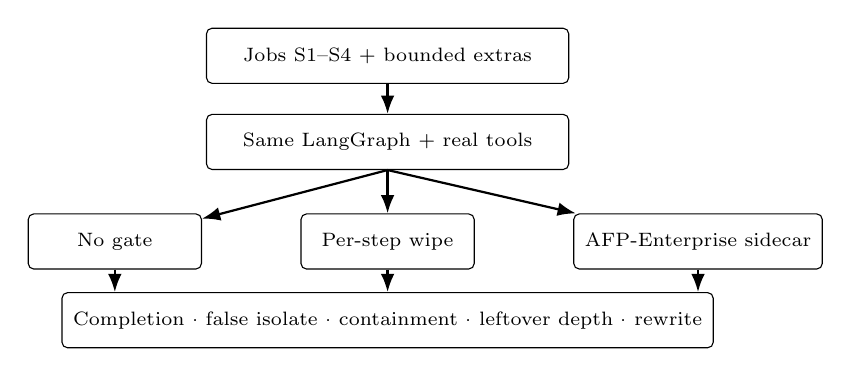
\begin{tikzpicture}[
  font=\scriptsize,
  box/.style={draw, rounded corners=2pt, align=center, inner sep=4pt, minimum height=0.70cm},
  arr/.style={-{Latex}, thick}
]
\node[box, minimum width=4.6cm] (jobs) {Jobs S1--S4 + bounded extras};
\node[box, below=0.38cm of jobs, minimum width=4.6cm] (graph) {Same LangGraph + real tools};
\node[box, below left=0.55cm and 0.05cm of graph, minimum width=2.2cm] (off) {No gate};
\node[box, below=0.55cm of graph, minimum width=2.2cm] (wipe) {Per-step wipe};
\node[box, below right=0.55cm and 0.05cm of graph, minimum width=2.2cm] (side) {AFP-Enterprise sidecar};
\node[box, below=1.55cm of graph, minimum width=7.4cm] (cons) {Completion · false isolate · containment · leftover depth · rewrite};
\draw[arr] (jobs) -- (graph);
\draw[arr] (graph.south) -- (off);
\draw[arr] (graph) -- (wipe);
\draw[arr] (graph.south) -- (side);
\draw[arr] (off.south) -- (cons.north -| off);
\draw[arr] (wipe) -- (cons);
\draw[arr] (side.south) -- (cons.north -| side);
\end{tikzpicture}
\caption{Same graph and tools. The three conditions differ only in whether leftover host telemetry is absent, wiped, or retained by AFP-Enterprise.}
\label{fig:design}
\end{figure}

\section{Results}
\label{sec:results}

\subsection{Reliability and first-time containment}
\label{sec:main}

Table~\ref{tab:trace} reports no-gate versus current sidecar on the four named jobs.
S1 and S2 finish with the gate on (false isolate $=0$ on those jobs).
S3 without the gate walks to the graph cap (depth $40$, $39$ ticks); with it, isolation fires at reported depth $11$.
S4 without the gate performs the expand plus $48$ GETs ($49$ tool executions); with it, the burst hint opens the breaker at entropy $0.96$ and no GET runs.

\begin{table}[htbp]
\caption{No-gate versus current sidecar on real tool I/O. S4 off, Tools $=49$: one expand plus $48$ GETs. A per-step wipe matches the sidecar on these four jobs (Table~\ref{tab:threeway}).}
\label{tab:trace}
\centering
{\small
\begin{tabular}{@{}llcccccl@{}}
\toprule
Job & Gate & Done & Tools & Probes & Isolated & Depth & Reason \\
\midrule
S1 short & off & yes & 1 & 0 & no & 2 & --- \\
S1 short & on & yes & 1 & 3 & no & 2 & --- \\
S2 long & off & yes & 8 & 0 & no & 9 & --- \\
S2 long & on & yes & 8 & 17 & no & 9 & --- \\
S3 runaway & off & to cap & 39 & 0 & no & 40 & --- \\
S3 runaway & on & no & 10 & 22 & yes & 11 & recursion cap \\
S4 storm & off & yes & 49 & 0 & no & 50 & --- \\
S4 storm & on & no & 0 & 2 & yes & 1 & burst entropy \\
\bottomrule
\end{tabular}
}
\end{table}

Bounded completion extends to five jobs: S1, S2, lookups only, fetches only, and eight repeats of one lookup.
All five complete under no gate, the wipe, and the current sidecar.
False isolate on that set is $0$.
In these local controlled runs, mean wall-clock on the five bounded jobs was $3.8$\,ms off and $6.0$--$6.4$\,ms gated.
That measurement is indicative only.
It is not a throughput or scalability benchmark.

\subsection{Where the gated variants differ}
\label{sec:threeway}

Table~\ref{tab:threeway} is the result that a gate-versus-off table conceals.
S1--S4 do not distinguish the two gated variants.
Both contain the loop and the burst; neither false-isolates the bounded set.
They differ only when a later execution reuses stale, uncleared telemetry: the current sidecar refuses; the wipe allows.
A new S1 that reports depth $0$ completes under both.
Appendix~\ref{app:baseline} lists every job under all three gates from the latest three-way run, including lookups only, fetches only, and eight repeats.

\begin{table}[htbp]
\caption{Three-way baseline. Bounded jobs complete under every gate. The gated columns differ only on a stale post-isolate probe.}
\label{tab:threeway}
\centering
\begin{tabular}{@{}lccc@{}}
\toprule
Scene & No gate & Per-step wipe & Current sidecar \\
\midrule
Five bounded jobs & done & done & done \\
False isolate & $0$ & $0$ & $0$ \\
Infinite loop / 48-burst & not stopped & stopped & stopped \\
Stale probe, no rewrite & --- & allow & \textbf{refuse} \\
New job reports depth $0$ & --- & allow & allow \\
\bottomrule
\end{tabular}
\end{table}

This is evidence for leftover telemetry, not for a penalty locked to agent identity.
After S3 isolate, a probe that does not rewrite depth is still refused by the current sidecar; a new graph that reports depth $0$ is admitted.
Request completion alone does not clear leftover depth.
A later report of depth $0$ does.

State ownership fails on a shared sidecar.
Two planners on separate sidecars keep the second planner healthy while the first isolates on S3.
On one shared sidecar, the second planner's fresh report overwrites the first planner's leftover depth, and the second planner completes S1 (Appendix~\ref{app:stale}).
Isolation is a host-level check, not a per-agent record.
If two planners must not affect each other, they need separate sidecars, or the kernel must account per identity first.

A local Qwen2.5 0.5B completes S1 and does not finish S2 (Appendix~\ref{app:live}).
That is a model-quality result, not LLM-agent validation.
The scripted planner remains the primary evidence.

\section{Limitations}
\label{sec:limitations}

The evidence is a controlled planner--tool environment on one machine.
It is not computer-use, MCP ingress, injection robustness, multi-agent isolation, or production safety.
The primary planner is scripted; the live 0.5B arm does not finish the long recipe.
Jobs are deterministic, so the tables have no confidence intervals.
Latency is indicative only.
State ownership fails on a shared sidecar.
The emergency stop, the delay band, and the isolate--recover machine were not reached.
These traces stop a false persistence claim; they are not a complete runtime-safety benchmark.

\section{Conclusion}
\label{sec:conclusion}

Ordinary admission control decides from current resource state and forgets at request end.
AFP-Enterprise's measured distinction is leftover host telemetry on later pre-flight probes.
On the jobs that were tested, bounded work can finish, and a loop or burst can be stopped by the depth cap or the hard pressure isolate; a per-step wipe can do the same.
The gated variants differ only on a stale probe.
The delay band and the isolate--recover machine are specified; they are not evidenced by these tables.
That is the claim---not production safety, not multi-agent isolation, and not a lock on agent identity.

\aesbackmattersection{Ethics Statement}
This work records AFP-Enterprise on scripted and small-model planner--tool jobs.
It does not involve human subjects, user data, or production traffic.
The paper reports negative and bounding results (no difference on S1--S4 between the gated variants; failed state ownership; mesh $100\%$ as an invariant) so that the traces cannot be read as field safety.

\bibliography{references}

\appendix
\section{Stale telemetry and two planners}
\label{app:stale}

Isolation follows last-reported host telemetry on one sidecar, not a lock on agent identity.
Table~\ref{tab:persist} is the rewrite check after S3 isolate.
Table~\ref{tab:two} is the ownership check.

\begin{table}[htbp]
\centering
\caption{Same sidecar after S3 isolate. A stale probe keeps leftover depth $11$; a new S1 reports $0$ and overwrites it.}
\label{tab:persist}
\begin{tabular}{@{}lcccc@{}}
\toprule
Arm & Isolated & S1 done & Leftover depth & Reason \\
\midrule
Stale probe (no rewrite) & yes & --- & $11$ & recursion cap \\
Fresh S1 (reports depth $0$) & no & yes & $0$ & --- \\
\bottomrule
\end{tabular}
\end{table}

\begin{table}[htbp]
\centering
\caption{Two local planners. Split sidecars keep B healthy; a shared sidecar lets B overwrite A's telemetry. A's S3 is $10$ tools / $22$ probes; B's S1 is $1$ tool / $3$ probes in both layouts.}
\label{tab:two}
\begin{tabular}{@{}llccc@{}}
\toprule
Layout & Agent & Job & Isolated & Done \\
\midrule
Split sidecars & A & S3 & yes & no \\
Split sidecars & B & S1 & no & yes \\
Shared sidecar & A & S3 & yes & no \\
Shared sidecar & B & S1 & no & yes \\
\bottomrule
\end{tabular}
\end{table}

\section{Live run on a local small model}
\label{app:live}

Table~\ref{tab:live} uses Qwen2.5 0.5B via a local OpenAI-compatible endpoint, the same graph, and the same tools.
S1 is the only completed live job ($604$ prompt tokens in both modes).
S2 without the gate hits LangGraph \texttt{recursion\_limit}$=30$ with $0$ tools and $18{,}859$ prompt tokens.
S2 with the gate isolates a looping planner at depth $11$ ($10$ tools, $10{,}799$ prompt tokens).
Neither cell is a false isolate of a finished eight-tool job.
Live wall-clock is model-bound and is not used as an overhead figure.

\begin{table}[htbp]
\centering
\caption{Live AFP-Enterprise on Qwen2.5 0.5B. Supplementary only.}
\label{tab:live}
{\small
\begin{tabular}{@{}llccccc@{}}
\toprule
Job & Gate & Done & Tools & Isolated & Tokens & Reason \\
\midrule
S1 short & off & yes & 1 & no & $604$ & --- \\
S1 short & on & yes & 1 & no & $604$ & --- \\
S2 long & off & no & 0 & no & $18{,}859$ & graph \texttt{recursion\_limit}$=30$ \\
S2 long & on & no & 10 & yes & $10{,}799$ & recursion cap \\
\bottomrule
\end{tabular}
}
\end{table}

\section{Depth-only unit check}
\label{app:synth-depth}

Before tools were wired, the same sidecar isolated a depth-only planner (no lookup, no HTTP) at the recursion cap.
Table~\ref{tab:synth-depth} is that check; Table~\ref{tab:trace} is the main tool result.

\begin{table}[htbp]
\centering
\caption{Depth-only LangGraph (no tool I/O). Unit check, not the main evidence.}
\label{tab:synth-depth}
{\small
\begin{tabular}{@{}llcccccl@{}}
\toprule
Job & Gate & Finished & Steps & Probes & Isolated & Depth & Reason \\
\midrule
Benign & off & yes & 3 & 0 & no & 3 & --- \\
Benign & on & yes & 3 & 3 & no & 3 & --- \\
Runaway & off & to cap & 40 & 0 & no & 40 & --- \\
Runaway & on & no & 11 & 12 & yes & 11 & recursion cap \\
\bottomrule
\end{tabular}
}
\end{table}

\section{Three-way baseline, full latest run}
\label{app:baseline}

Table~\ref{tab:baseline} restates Table~\ref{tab:threeway} by gate.
Table~\ref{tab:baseline-jobs} is the latest three-way CSV: every bounded job, S3, S4, and the two post-isolate probes, under all three gates.
Mean wall-clock on the five bounded jobs is $3.8$\,ms off, $6.4$\,ms wipe, and $6.0$\,ms current sidecar; indicative only.

\begin{table}[htbp]
\centering
\caption{Three-way baseline by gate. Bounded jobs: $5/5$ complete, false isolate $=0$.}
\label{tab:baseline}
\begin{tabular}{@{}lcccc@{}}
\toprule
Gate & Bounded done & S3/S4 isolated & Stale probe & Fresh S1 \\
\midrule
Off & $5/5$ & $0/2$ & --- & --- \\
Per-step wipe & $5/5$ & $2/2$ & allow & done \\
Current sidecar & $5/5$ & $2/2$ & refuse & done \\
\bottomrule
\end{tabular}
\end{table}

\begin{table}[htbp]
\centering
\caption{Latest three-way run (scripted planner, real tools). Wipe matches the current sidecar on every job row; they differ only on the stale probe.}
\label{tab:baseline-jobs}
{\scriptsize
\begin{tabular}{@{}llcccccl@{}}
\toprule
Job & Gate & Done & Tools & Probes & Isolated & Wall (ms) & Reason \\
\midrule
S1 short & off & yes & 1 & 0 & no & $1.6$ & --- \\
S1 short & wipe & yes & 1 & 3 & no & $2.0$ & --- \\
S1 short & sidecar & yes & 1 & 3 & no & $2.0$ & --- \\
S2 long & off & yes & 8 & 0 & no & $8.3$ & --- \\
S2 long & wipe & yes & 8 & 17 & no & $9.4$ & --- \\
S2 long & sidecar & yes & 8 & 17 & no & $8.7$ & --- \\
Lookups only & off & yes & 4 & 0 & no & $1.5$ & --- \\
Lookups only & wipe & yes & 4 & 9 & no & $3.8$ & --- \\
Lookups only & sidecar & yes & 4 & 9 & no & $4.2$ & --- \\
Fetches only & off & yes & 6 & 0 & no & $5.3$ & --- \\
Fetches only & wipe & yes & 6 & 13 & no & $10.3$ & --- \\
Fetches only & sidecar & yes & 6 & 13 & no & $8.4$ & --- \\
Eight repeats & off & yes & 8 & 0 & no & $2.1$ & --- \\
Eight repeats & wipe & yes & 8 & 17 & no & $6.3$ & --- \\
Eight repeats & sidecar & yes & 8 & 17 & no & $6.7$ & --- \\
S3 runaway & off & yes & 39 & 0 & no & $8.3$ & --- \\
S3 runaway & wipe & no & 10 & 22 & yes & $7.9$ & recursion cap \\
S3 runaway & sidecar & no & 10 & 22 & yes & $8.1$ & recursion cap \\
S4 storm & off & yes & 49 & 0 & no & $30.8$ & --- \\
S4 storm & wipe & no & 0 & 2 & yes & $1.5$ & burst entropy \\
S4 storm & sidecar & no & 0 & 2 & yes & $1.9$ & burst entropy \\
Stale probe & wipe & --- & 0 & 1 & no & --- & allow after wipe \\
Stale probe & sidecar & --- & 0 & 1 & yes & --- & recursion cap \\
Fresh S1 & wipe & yes & 1 & 3 & no & --- & reports depth $0$ \\
Fresh S1 & sidecar & yes & 1 & 3 & no & --- & reports depth $0$ \\
\bottomrule
\end{tabular}
}
\end{table}

\section{Synthetic mesh: an invariant, not a field result}
\label{app:mesh}

Death is defined as load $\ge 1$.
The simulated gate refuses any request with $\mathrm{load}+\mathrm{request}>0.95$.
Under that pair of rules a node cannot die: $100\%$ survival is an invariant of the construction.
The complementary fact is that without any pre-accumulation refusal, the same seeds collapse (mean $1.876/500$ alive at $T=100$ over $1{,}000$ runs).
Viability $v$ is a floor used only in this simulated mesh; it is not part of the LangGraph sidecar traces.
Table~\ref{tab:ablate} locates the invariant in the breaker, not in $v$.
Tables~\ref{tab:rate} and~\ref{tab:adapt} are the same invariant under a malicious-rate sweep and a reduced per-request load.
The $100\%$ cells are an invariant of the construction, not a field result.

\begin{table}[htbp]
\centering
\caption{Mean survival (\%) at $T=100$. Breaker-only matches the full gate; viability-only matches baseline.}
\label{tab:ablate}
\begin{tabular}{@{}lcccccc@{}}
\toprule
Malicious \% & Full & No $v$ floor & No breaker & No burst tax & Breaker only & $v$ only / base \\
\midrule
$5$  & $100$ & $100$ & $4.8$  & $100$ & $100$ & $0.3$ / $0.3$ \\
$20$ & $100$ & $100$ & $15.7$ & $100$ & $100$ & $0.2$ / $0.2$ \\
\bottomrule
\end{tabular}
\end{table}

\begin{table}[htbp]
\centering
\caption{Mean survival (\%) at $T=100$ versus malicious fraction ($300$ runs). Every full-gate cell is the breaker invariant.}
\label{tab:rate}
{\small
\begin{tabular}{@{}lcccccccc@{}}
\toprule
Mode & $1\%$ & $5\%$ & $10\%$ & $15\%$ & $20\%$ & $30\%$ & $40\%$ & $50\%$ \\
\midrule
Baseline & $2.3$ & $0.3$ & $0.3$ & $0.3$ & $0.2$ & $0.2$ & $0.2$ & $0.2$ \\
Full gate & $100$ & $100$ & $100$ & $100$ & $100$ & $100$ & $100$ & $100$ \\
\bottomrule
\end{tabular}
}
\end{table}

\begin{table}[htbp]
\centering
\caption{Mean survival (\%) when malicious per-request load is reduced ($5\%$ malicious, $300$ runs).}
\label{tab:adapt}
\begin{tabular}{@{}lcccc@{}}
\toprule
Malicious load & $0.80$ & $0.45$ & $0.20$ & $0.12$ \\
\midrule
Baseline & $0.3$ & $0.6$ & $3.1$ & $7.8$ \\
Full gate & $100$ & $100$ & $100$ & $100$ \\
\bottomrule
\end{tabular}
\end{table}

\end{document}
